\documentclass{article}

% Requires the official NeurIPS 2026 style file: neurips_2026.sty.
% Upload neurips_2026.sty from the official NeurIPS 2026 Overleaf template if it is
% not already present in this folder.
\usepackage[preprint]{neurips_2026}

\usepackage[utf8]{inputenc}
\usepackage[T1]{fontenc}
\usepackage{hyperref}
\usepackage{url}
\usepackage{booktabs}
\usepackage{graphicx}
\usepackage{amsfonts}
\usepackage{nicefrac}
\usepackage{microtype}
\usepackage{xcolor}

\title{Emotion Recognition from Facial Expressions using CNNs, Transfer Learning, and Foundation Models}

\author{%
  Anirudh Ramesh \\
  Department of Computer Science and Engineering\\
  University at Buffalo\\
  CSE 676 Deep Learning, Spring 2026\\
  \And
  Rohan Marar \\
  Department of Computer Science and Engineering\\
  University at Buffalo\\
  CSE 676 Deep Learning, Spring 2026\\
}

\begin{document}

\maketitle

\begin{abstract}
We study facial emotion recognition on FER-2013, a benchmark of low-resolution face images labeled with seven emotion classes. The project compares a baseline convolutional network, ResNet-18 transfer learning, EfficientNet-B0, ConvNeXt-Tiny, CLIP-based foundation-model experiments, cleaned-data training, test-time augmentation, and soft-voting ensembles. The best final model was a CLIP + cleaned-data ensemble with 70.23\% test accuracy, improving over the cleaned-data ensemble at 69.77\%. Standalone CLIP did not outperform the strongest CNN-based models, but it contributed complementary probability estimates when combined with the cleaned-data ensemble. We also built a Streamlit demo that supports image upload, webcam photo capture, and live webcam inference from saved checkpoints.
\end{abstract}

\section{Introduction}

Facial emotion recognition (FER) aims to classify a face image into an expression category such as happy, sad, angry, or surprised. It is useful for human-computer interaction, affective computing, accessibility, and educational prototypes \citep{li2020deep}, but it is also a difficult visual recognition task. Expressions are subtle, people show emotions differently, and the same label can correspond to a wide range of facial appearances.

Our project uses FER-2013, introduced through the ICML representation learning challenge \citep{goodfellow2013challenges}. FER-2013 is challenging because the images are only 48$\times$48 grayscale pixels, labels are noisy, the classes are imbalanced, and several categories overlap visually. Fear is often confused with sad or angry, while sad and neutral can be difficult to separate. For this reason, our goal was not to tune a single model in isolation. Instead, we compared several learning strategies: a custom CNN, ImageNet transfer learning, modern CNN backbones, CLIP foundation-model features, cleaned-data training, and ensembles.

\section{Dataset and preprocessing}

FER-2013 contains about 35,887 facial images across seven classes: Angry, Disgust, Fear, Happy, Neutral, Sad, and Surprise \citep{kagglefer2013}. The local ImageFolder layout used 28,709 training images and 7,178 test images. Since the downloaded archive did not include a separate validation folder, the notebooks used an 80/20 split of the training folder for training and validation. The held-out test folder was kept separate for final evaluation.

For the baseline CNN, images were loaded as grayscale tensors and normalized for training from scratch. For ResNet-18, EfficientNet-B0, and ConvNeXt-Tiny, grayscale images were converted to RGB, resized to 224$\times$224, converted to tensors, and normalized with ImageNet mean and standard deviation. CLIP used RGB 224$\times$224 inputs with CLIP normalization. Augmentations included random horizontal flips, small rotations, affine shifts, color jitter where appropriate, and normalization. Class imbalance was handled with inverse-frequency class weights in cross-entropy loss. The notebooks also included cleaned-data experiments that removed a conservative set of high-confidence label disagreements from the training subset, without changing validation or test labels.

\section{Methodology}

\subsection{Baseline CNN}

The baseline model was a small convolutional network trained from scratch on FER-2013. It used convolutional blocks with batch normalization, ReLU activations, max pooling, dropout, and a fully connected classifier. This model provided a simple reference point and reached about 57.4\%--57.7\% test accuracy depending on the run.

\subsection{ResNet-18 transfer learning}

We tested ImageNet-pretrained ResNet-18 \citep{he2016deep} in two stages. First, we froze the backbone and trained only the classifier head. This transferred poorly to FER-2013 and produced about 39.2\% test accuracy. A likely reason is that fixed ImageNet features are not specialized for low-resolution grayscale facial expressions. We then fine-tuned later layers, including deeper residual blocks and the classifier head, with class-weighted loss and smaller learning rates for the backbone. Fine-tuning improved performance substantially, reaching about 66.6\% in the checkpoint notebook and 67.32\% in the final comparison table.

\subsection{EfficientNet-B0 and ConvNeXt-Tiny}

EfficientNet-B0 \citep{tan2019efficientnet} was included as a stronger transfer-learning comparison, but it underperformed ResNet-18 fine-tuning in our runs. ConvNeXt-Tiny \citep{liu2022convnet} performed better and became the main CNN branch for later experiments. We also evaluated test-time augmentation (TTA) by averaging predictions over simple transformed versions of the same test image. The cleaned-data ConvNeXt run improved robustness, and a cleaned-data ensemble with a ResNet branch reached 69.77\% test accuracy.

For transfer-learning models such as EfficientNet-B0 and ConvNeXt-Tiny, we used ChatGPT only as a support tool to understand reasonable fine-tuning choices, such as which blocks to unfreeze, learning-rate ranges, and regularization options. The final settings were manually checked, run in Colab, and evaluated using notebook outputs.

\subsection{CLIP foundation model}

CLIP \citep{radford2021learning} was included because the course guidance asked us to use a foundation CLIP model. We evaluated zero-shot CLIP with prompts such as ``a photo of a happy face,'' then trained a linear probe and a lightly fine-tuned CLIP image encoder. Zero-shot CLIP was weak on FER-2013 because the inputs are grayscale, low resolution, and emotion-specific. Linear probing and light fine-tuning helped, but standalone CLIP still did not match the strongest CNN and cleaned-data models. Its value appeared in the final ensemble: CLIP probabilities added complementary information to the cleaned-data ensemble.

\subsection{Final ensemble and demo modes}

The final ensemble used soft voting by averaging class probabilities. This avoids averaging labels or logits and keeps each branch's distribution over the seven classes. The Streamlit app exposes two practical modes. Fast Mode uses cleaned-data ConvNeXt-Tiny for smoother live webcam inference. Best Mode uses the CLIP + cleaned-data ensemble when the required checkpoints are available.

\begin{figure}[t]
  \centering
  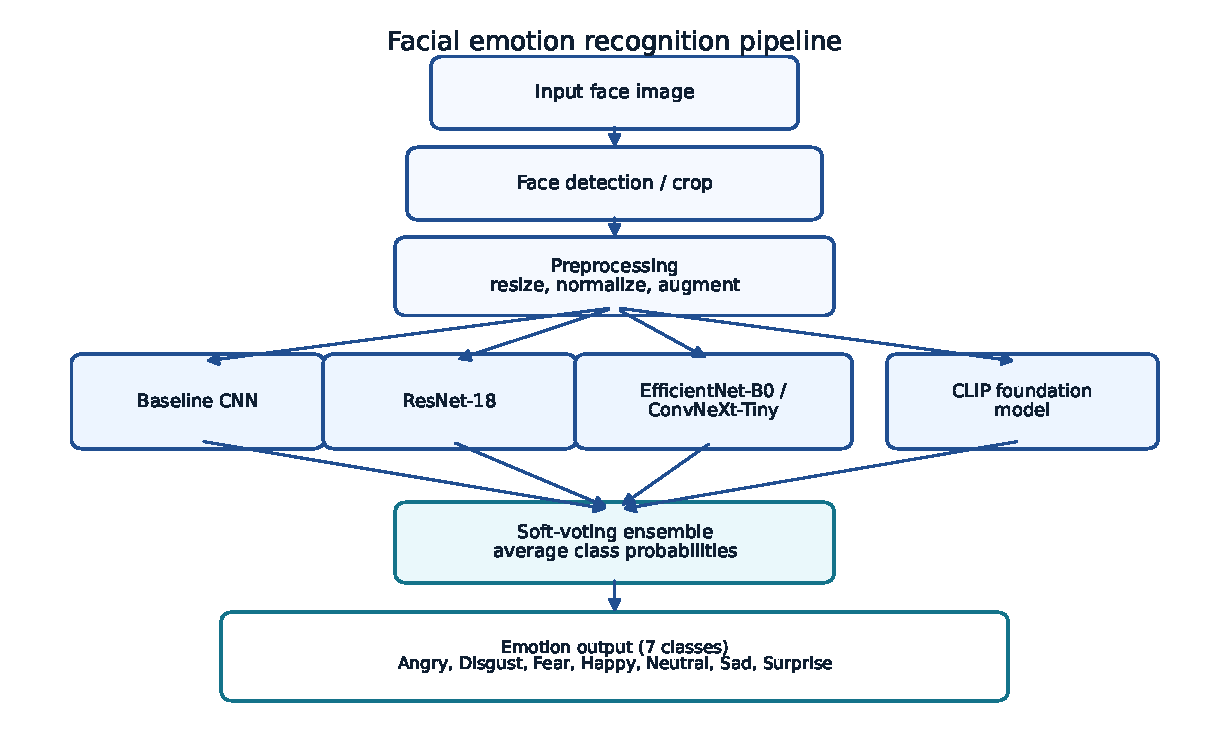
\includegraphics[width=0.95\linewidth]{figures/architecture_diagram.pdf}
  \caption{Overall pipeline of the facial emotion recognition system.}
  \label{fig:architecture}
\end{figure}

\section{Experimental setup}

Experiments were implemented in Python with PyTorch, torchvision, scikit-learn, and open\_clip\_torch. Training and evaluation were run on Google Colab Pro GPU; later final experiments used Colab Pro GPU resources, with stronger GPU runtimes when available. Optimizers included Adam for the baseline CNN and AdamW for transfer-learning and foundation-model fine-tuning. Several models used weighted cross-entropy, label smoothing where supported, mixed precision, learning-rate scheduling, early stopping, and test-time augmentation. We evaluated models with test accuracy, weighted F1, macro F1, precision, recall, classification reports, and confusion matrices where available.

\section{Results}

Table~\ref{tab:results} summarizes the main test results from the notebooks. Missing values are shown only when a metric was not available. The final comparison indicates that the CLIP + cleaned-data ensemble achieved the best test accuracy, while CLIP alone remained below the strongest CNN-based branches.

\begin{table}[t]
  \caption{FER-2013 test results from notebook evaluations.}
  \label{tab:results}
  \centering
  \small
  \begin{tabular}{lccc}
    \toprule
    Model & Accuracy & Weighted F1 & Macro F1 \\
    \midrule
    Baseline CNN & 0.5737 & 0.5573 & 0.5119 \\
    ResNet-18 Feature Extraction & 0.3924 & 0.3777 & 0.3356 \\
    ResNet-18 Fine-Tuning & 0.6732 & 0.6716 & 0.6566 \\
    EfficientNet-B0 & 0.5535 & 0.5593 & 0.4986 \\
    ConvNeXt-Tiny & 0.6645 & 0.6641 & 0.6308 \\
    ConvNeXt-Tiny + TTA & 0.6675 & 0.6673 & 0.6325 \\
    ResNet-18 + ConvNeXt Ensemble & 0.6889 & 0.6871 & 0.6672 \\
    Cleaned-data ConvNeXt-Tiny & 0.6785 & 0.6772 & 0.6419 \\
    Cleaned-data ConvNeXt-Tiny + TTA & 0.6787 & 0.6774 & 0.6415 \\
    Cleaned-data Ensemble & 0.6977 & 0.6970 & 0.6639 \\
    CLIP Zero-Shot & 0.2814 & 0.2824 & 0.2469 \\
    CLIP Linear Probe & 0.5995 & 0.6039 & 0.5288 \\
    CLIP Fine-Tuning & 0.6308 & 0.6369 & 0.5647 \\
    CLIP Fine-Tuning + TTA & 0.6342 & 0.6398 & 0.5677 \\
    CLIP + Cleaned-data Ensemble & \textbf{0.7023} & \textbf{0.7022} & 0.6501 \\
    \bottomrule
  \end{tabular}
\end{table}

\begin{figure}[t]
  \centering
  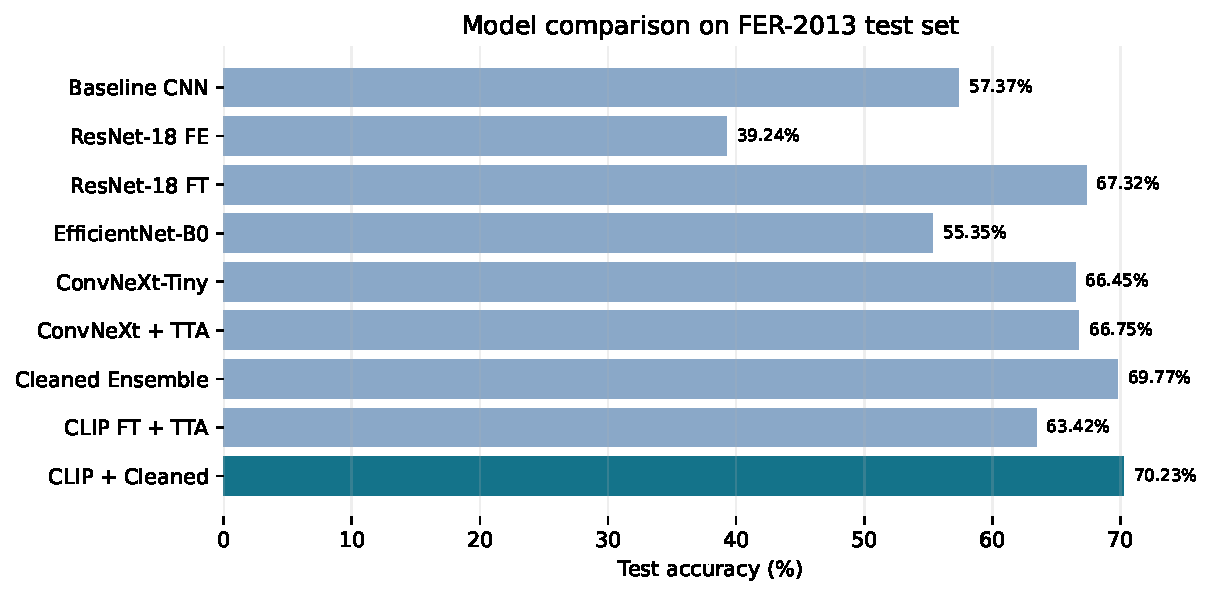
\includegraphics[width=0.94\linewidth]{figures/model_comparison.pdf}
  \caption{Test accuracy comparison for selected models. The best final result was the CLIP + cleaned-data ensemble.}
  \label{fig:comparison}
\end{figure}

\section{Discussion and error analysis}

The frozen ResNet-18 result shows that ImageNet features do not transfer directly to FER-2013 when the backbone is fixed. Fine-tuning later layers allowed the model to adapt to face-specific cues and improved the result by more than 25 percentage points. ConvNeXt-Tiny and cleaned-data training improved the strongest CNN branch, and probability averaging reduced some model-specific errors.

CLIP zero-shot performance was low, which is expected for this setting. CLIP is trained on image-text pairs at a much broader scale, but FER-2013 requires fine-grained emotion recognition from small grayscale face images. However, the final ensemble result suggests that CLIP captures information that is not identical to the CNN branches. This is why standalone CLIP was not the best model, but CLIP still helped the final ensemble.

Class-level errors followed expected FER-2013 patterns. Fear was frequently confused with sad or angry, sad and neutral overlapped, and disgust remained difficult because it has very few training samples. These issues are partly caused by class imbalance and partly by label ambiguity. The Streamlit demo also introduces practical sources of error such as webcam lighting, pose, face crop quality, and differences between live images and FER-2013.

\section{Streamlit demo and deployment}

We built a Streamlit demo \citep{streamlitdocs} with image upload, webcam photo capture, and live webcam inference. The app detects and crops the largest face, displays the crop that is sent to the model, and reports the predicted emotion, confidence, top-3 predictions, and all class probabilities. Fast Mode uses cleaned-data ConvNeXt-Tiny for smoother live inference. Best Mode loads the available cleaned-data and CLIP checkpoints and averages softmax probabilities. No training is performed inside the Streamlit app.

ChatGPT was referenced for Streamlit layout ideas and debugging guidance, but the app was manually connected to trained checkpoints, tested, and modified by the team.

\section{LLM usage statement}

LLM tools were used as a support resource during the project, mainly for brainstorming model extensions, understanding fine-tuning options for transfer-learning models, debugging notebook/runtime issues, and improving the organization of the Streamlit demo and final report. For example, we used ChatGPT to compare possible directions such as EfficientNet-B0, ConvNeXt, and CLIP fine-tuning, and to get suggestions on Streamlit layout/debugging. The CLIP foundation-model experiment was included based on course guidance. All training, evaluation, checkpoint generation, metric reporting, and final interpretation were completed and verified by the team using our Colab notebook outputs.

\section{Team contributions}

Anirudh Ramesh worked on the data setup, preprocessing flow, notebook organization, and final experiment tracking. He also handled the EfficientNet/ConvNeXt comparison work, cleaned-data and ensemble experiments, CLIP foundation-model experiments, CLIP fine-tuning and comparison framing, Streamlit demo integration, checkpoint-based inference setup, and final result interpretation.

Rohan Marar worked on the baseline CNN and ResNet-18 transfer-learning experiments, including feature extraction and fine-tuning comparisons. He also contributed to evaluation tables, plots, confusion-matrix analysis, checkpoint report material and figures, and the discussion of model behavior and limitations.

Both team members reviewed notebook outputs, checked the reported metrics against the saved results, and contributed to the final report and presentation narrative.

\textbf{GitHub Repository:} \url{https://github.com/Anir11/Facial-Emotion-Recognition}

\section{Ethics, privacy, and limitations}

Emotion recognition is sensitive and should not be used for high-stakes decisions. The model predicts labels from visual appearance, not a person's true internal state. Webcam use also raises privacy concerns, so the demo should be treated as an educational prototype. Predictions can be affected by dataset bias, lighting, pose, occlusion, and face crop quality. Future deployments would need consent, calibration, bias evaluation, and stronger privacy controls.

\section{Future work}

Future work could use AffectNet or RAF-DB pretraining, FER-specific pretrained backbones, better face detection and alignment, temporal smoothing for live video, improved class balancing, label-noise handling, model distillation, confidence calibration, and lighter deployment models for real-time use.

\section{Conclusion}

We built an end-to-end FER pipeline on FER-2013 and compared several model families. Fine-tuning was essential for transfer learning, ConvNeXt and cleaned-data training improved the strongest CNN results, and CLIP alone was not the best standalone model. The final CLIP + cleaned-data ensemble achieved about 70.23\% test accuracy, indicating that CLIP contributed complementary information when combined with the cleaned-data ensemble. The Streamlit app demonstrates practical saved-checkpoint inference for images, webcam photos, and live video.

\bibliographystyle{plainnat}
\bibliography{references}

\end{document}
